\section{Architecture}

	\begin{frame}{Master-Worker}
		\centerline{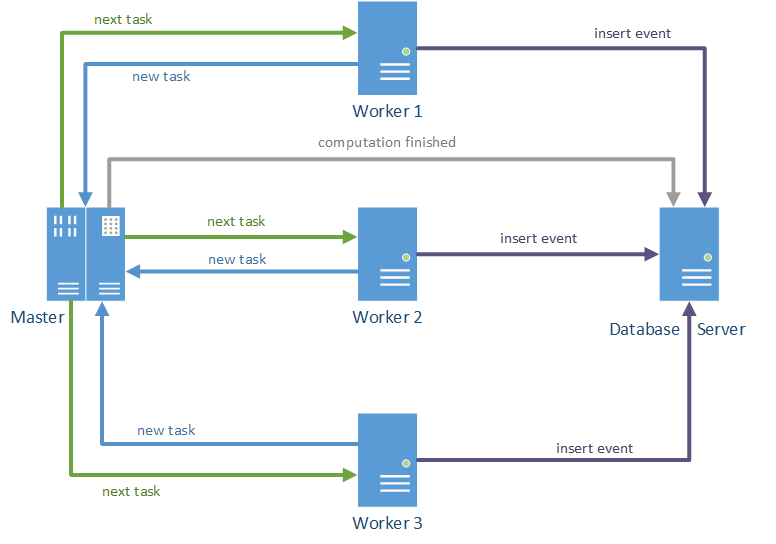
\includegraphics[scale=0.5]{images/master}}
	\end{frame}
	\begin{frame}{Task Stealing}
		\centerline{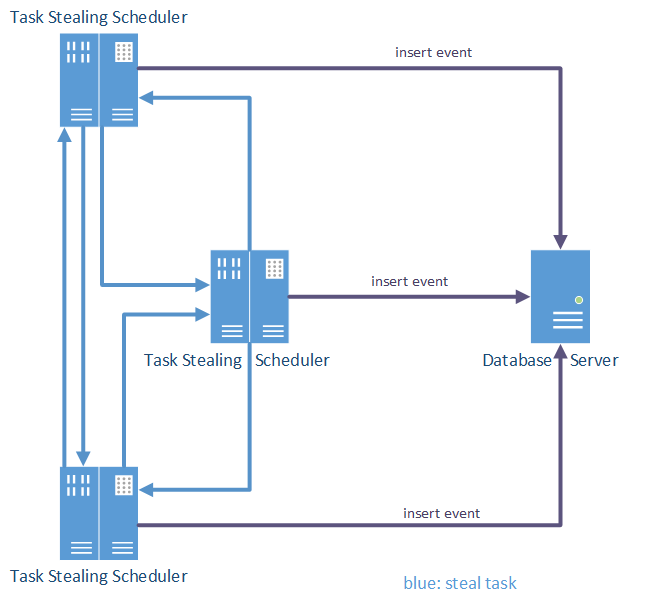
\includegraphics[scale=0.5]{images/taskstealing}}
	\end{frame}

	\begin{frame}{Scheduling strategies}
		\begin{itemize}
		\item non statistical
		\begin{itemize}
			\item First In-First out (FIFO)
			\item Last In-Last out
		\end{itemize}
		\item statistical
		\begin{itemize}
			\item Shortest job first
			\item Longest job first
		\end{itemize}
		\item standardized interface - it is very easy to include new strategies
		\end{itemize}
	\end{frame}
	\begin{frame}{Scheduling strategies: Master-Worker vs. Task stealing}
		\begin{itemize}
			\item Master-Worker
				\begin{itemize}
					\item fast standard c++ implementation
					\item dynamically size
					\item easy to switch between scheduling strategies online					
				\end{itemize}
			
			\item Task stealing
					\begin{itemize}
						\item own implementation in MPI-Window
						\item synchronization overhead
					\end{itemize}
			
		\end{itemize}
	\end{frame}